% 本模板根据中国科学院大学本科生公共必修课程《基础物理实验》Word模板格式编写
% 本模板由Shing-Ho Lin和Jun-Xiong Ji于2022年9月共同完成, 旨在方便LaTeX原教旨主义者和被Word迫害者写实验报告, 避免Word文档因插入过多图与公式造成卡顿. 
% 如有任何问题, 请联系: linchenghao21@mails.ucas.ac.cn
% This is the LaTeX template for experiment report of Experimental Physics courses, based on its provided Word template. 
% This template is completed by the joint collabration of Shing-Ho Lin and Junxiong Ji in September 2022. 
% Adding numerous pictures and equations leads to unsatisfying experience in Word. Therefore LaTeX is better. 
% Feel free to contact us via: linchenghao21@mails.ucas.ac.cn

\documentclass[11pt]{article}

\usepackage[a4paper]{geometry}
\geometry{left=2.0cm,right=2.0cm,top=2.5cm,bottom=2.5cm}

\usepackage{ctex} % 支持中文的LaTeX宏包
\usepackage{amsmath,amsfonts,graphicx,subfigure,amssymb,bm,amsthm,mathrsfs,mathtools,breqn} % 数学公式和符号的宏包集合
\usepackage{algorithm,algorithmicx} % 算法和伪代码的宏包
\usepackage[noend]{algpseudocode} % 算法和伪代码的宏包
\usepackage{fancyhdr} % 自定义页眉页脚的宏包
\usepackage[framemethod=TikZ]{mdframed} % 创建带边框的框架的宏包
\usepackage{fontspec} % 字体设置的宏包
\usepackage{adjustbox} % 调整盒子大小的宏包
\usepackage{fontsize} % 设置字体大小的宏包
\usepackage{tikz,xcolor} % 绘制图形和使用颜色的宏包
\usepackage{multicol} % 多栏排版的宏包
\usepackage{multirow} % 表格中合并单元格的宏包
\usepackage{pdfpages} % 插入PDF文件的宏包
\RequirePackage{listings} % 在文档中插入源代码的宏包
\RequirePackage{xcolor} % 定义和使用颜色的宏包
\usepackage{wrapfig} % 文字绕排图片的宏包
\usepackage{bigstrut,multirow,rotating} % 支持在表格中使用特殊命令的宏包
\usepackage{booktabs} % 创建美观的表格的宏包
\usepackage{circuitikz} % 绘制电路图的宏包

\definecolor{dkgreen}{rgb}{0,0.6,0}
\definecolor{gray}{rgb}{0.5,0.5,0.5}
\definecolor{mauve}{rgb}{0.58,0,0.82}
\lstset{
  frame=tb,
  aboveskip=3mm,
  belowskip=3mm,
  showstringspaces=false,
  columns=flexible,
  framerule=1pt,
  rulecolor=\color{gray!35},
  backgroundcolor=\color{gray!5},
  basicstyle={\small\ttfamily},
  numbers=none,
  numberstyle=\tiny\color{gray},
  keywordstyle=\color{blue},
  commentstyle=\color{dkgreen},
  stringstyle=\color{mauve},
  breaklines=true,
  breakatwhitespace=true,
  tabsize=3,
}

% 轻松引用, 可以用\cref{}指令直接引用, 自动加前缀. 
% 例: 图片label为fig:1
% \cref{fig:1} => Figure.1
% \ref{fig:1}  => 1
\usepackage[capitalize]{cleveref}
% \crefname{section}{Sec.}{Secs.}
\Crefname{section}{Section}{Sections}
\Crefname{table}{Table}{Tables}
\crefname{table}{Table.}{Tabs.}

\setmainfont{Palatino Linotype.ttf}
\setCJKmainfont{SimHei.ttf}
% \setCJKsansfont{Songti.ttf}
% \setCJKmonofont{SimSun.ttf}
\punctstyle{kaiming}
% 偏好的几个字体, 可以根据需要自行加入字体ttf文件并调用

\renewcommand{\emph}[1]{\begin{kaishu}#1\end{kaishu}}

%改这里可以修改实验报告表头的信息
\newcommand{\experiName}{将大象装进冰箱}
\newcommand{\supervisor}{Jun-Xiong Ji}
\newcommand{\name}{Shing-Ho}
\newcommand{\studentNum}{20xxK800xxxxxxx}
\newcommand{\class}{x}
\newcommand{\group}{xx}
\newcommand{\seat}{x}
\newcommand{\dateYear}{20xx}
\newcommand{\dateMonth}{xx}
\newcommand{\dateDay}{xx}
\newcommand{\room}{xxx}
\newcommand{\others}{$\square$}
%% 如果是调课、补课, 改为: $\square$\hspace{-1em}$\surd$
%% 否则, 请用: $\square$
%%%%%%%%%%%%%%%%%%%%%%%%%%%

\begin{document}

%若需在页眉部分加入内容, 可以在这里输入
% \pagestyle{fancy}
% \lhead{\kaishu 测试}
% \chead{}
% \rhead{}

\begin{center}
    \LARGE \bf 《\, 基\, 础\, 物\, 理\, 实\, 验\, 》\, 实\, 验\, 报\, 告
\end{center}

\begin{center}
    \noindent \emph{实验名称}\underline{\makebox[25em][c]{\experiName}}
    \emph{指导教师}\underline{\makebox[8em][c]{\supervisor}}\\
    \emph{姓名}\underline{\makebox[6em][c]{\name}} 
    % 如果名字比较长, 可以修改box的长度"6em"
    \emph{学号}\underline{\makebox[10em][c]{\studentNum}}
    \emph{分班分组及座号} \underline{\makebox[5em][c]{\class \ -\ \group \ -\ \seat }\emph{号}} (\emph{例}:\, 1\,-\,04\,-\,5\emph{号})\\
    \emph{实验日期} \underline{\makebox[3em][c]{\dateYear}}\emph{年}
    \underline{\makebox[2em][c]{\dateMonth}}\emph{月}
    \underline{\makebox[2em][c]{\dateDay}}\emph{日}
    \emph{实验地点}\underline{{\makebox[4em][c]\room}}
    \emph{调课/补课} \underline{\makebox[3em][c]{\others\ 是}}
    \emph{成绩评定} \underline{\hspace{5em}}
    {\noindent}
    \rule[8pt]{17cm}{0.2em}
\end{center}

\begin{center}
    \Large \bf 第一部分\qquad 把大象放进冰箱
\end{center}

\section{实验目的}

\begin{enumerate}
    \item 掌握冰箱的使用
    \item 掌握大象的搬运
    \item 了解冰淇淋的吃法
    \item 放弃使用Word写实验报告
\end{enumerate}

\section{实验器材}

overleaf, \LaTeX

\section{仪器用具}

冰箱、大象、冰淇淋

\begin{enumerate}
    \item 冰箱
    \begin{enumerate}
        \item 冰箱冰箱冰箱冰箱冰箱冰箱冰箱冰箱冰箱冰箱冰箱冰箱冰箱冰箱冰箱冰箱冰箱冰箱冰箱冰箱冰箱冰箱冰箱冰箱冰箱冰箱冰箱冰箱冰箱冰箱冰箱冰箱冰箱冰箱冰箱冰箱冰箱冰箱冰箱冰箱冰箱冰箱冰箱冰箱冰箱冰箱冰箱冰箱冰箱冰箱冰箱冰箱冰箱冰箱冰箱冰箱冰箱冰箱冰箱冰箱冰箱冰箱冰箱冰箱冰箱冰箱冰箱冰箱冰箱冰箱冰箱冰箱冰箱冰箱冰箱冰箱冰箱冰箱冰箱冰箱冰箱冰箱冰箱冰箱冰箱冰箱
        \item 冰箱冰箱冰箱冰箱冰箱冰箱冰箱冰箱冰箱冰箱冰箱冰箱冰箱冰箱冰箱冰箱冰箱冰箱冰箱冰箱冰箱冰箱冰箱冰箱冰箱冰箱冰箱冰箱冰箱冰箱冰箱冰箱冰箱冰箱冰箱冰箱冰箱冰箱冰箱冰箱冰箱冰箱冰箱冰箱冰箱冰箱冰箱冰箱冰箱冰箱冰箱冰箱冰箱冰箱冰箱冰箱冰箱冰箱冰箱冰箱冰箱冰箱冰箱冰箱冰箱冰箱冰箱冰箱冰箱冰箱冰箱冰箱冰箱冰箱冰箱冰箱冰箱冰箱冰箱冰箱冰箱冰箱冰箱冰箱冰箱冰箱
        \item 冰箱冰箱冰箱冰箱冰箱冰箱冰箱冰箱冰箱冰箱冰箱冰箱冰箱冰箱冰箱冰箱冰箱冰箱冰箱冰箱冰箱冰箱冰箱冰箱冰箱冰箱冰箱冰箱冰箱冰箱冰箱冰箱冰箱冰箱冰箱冰箱冰箱冰箱冰箱冰箱冰箱冰箱冰箱冰箱冰箱冰箱冰箱冰箱冰箱冰箱冰箱冰箱冰箱冰箱冰箱冰箱冰箱冰箱冰箱冰箱冰箱冰箱冰箱冰箱冰箱冰箱冰箱冰箱冰箱冰箱冰箱冰箱冰箱冰箱冰箱冰箱冰箱冰箱冰箱冰箱冰箱冰箱冰箱冰箱冰箱冰箱
    \end{enumerate}
    \item 大象
    \begin{enumerate}
        \item 大象大象大象大象大象大象大象大象大象大象大象大象大象大象大象大象大象大象大象大象大象大象大象大象大象大象大象大象大象大象大象大象大象大象大象大象大象大象大象大象大象大象大象大象大象大象大象大象大象大象大象大象大象大象大象大象大象大象大象大象大象大象大象大象大象大象大象大象大象大象大象大象大象大象大象大象大象大象大象大象大象大象大象大象大象大象
        \item 大象大象大象大象大象大象大象大象大象大象大象大象大象大象大象大象大象大象大象大象大象大象大象大象大象大象大象大象大象大象大象大象大象大象大象大象大象大象大象大象大象大象大象大象大象大象大象大象大象大象大象大象大象大象大象大象大象大象大象大象大象大象大象大象大象大象大象大象大象大象大象大象大象大象大象大象大象大象大象大象大象大象大象大象大象大象
        \item 大象大象大象大象大象大象大象大象大象大象大象大象大象大象大象大象大象大象大象大象大象大象大象大象大象大象大象大象大象大象大象大象大象大象大象大象大象大象大象大象大象大象大象大象大象大象大象大象大象大象大象大象大象大象大象大象大象大象大象大象大象大象大象大象大象大象大象大象大象大象大象大象大象大象大象大象大象大象大象大象大象大象大象大象大象大象
    \end{enumerate}
    \item 冰淇淋
    \begin{enumerate}
        \item 冰淇淋冰淇淋冰淇淋冰淇淋冰淇淋冰淇淋冰淇淋冰淇淋冰淇淋冰淇淋冰淇淋冰淇淋冰淇淋冰淇淋冰淇淋冰淇淋冰淇淋冰淇淋冰淇淋冰淇淋冰淇淋冰淇淋冰淇淋冰淇淋冰淇淋冰淇淋冰淇淋冰淇淋冰淇淋冰淇淋冰淇淋冰淇淋冰淇淋冰淇淋冰淇淋冰淇淋冰淇淋冰淇淋冰淇淋冰淇淋冰淇淋冰淇淋冰淇淋冰淇淋冰淇淋冰淇淋冰淇淋冰淇淋冰淇淋冰淇淋冰淇淋冰淇淋冰淇淋冰淇淋冰淇淋冰淇淋冰淇淋
        \begin{enumerate}
            \item 冰淇淋冰淇淋冰淇淋冰淇淋冰淇淋冰淇淋冰淇淋冰淇淋冰淇淋冰淇淋冰淇淋冰淇淋冰淇淋冰淇淋冰淇淋冰淇淋冰淇淋冰淇淋冰淇淋冰淇淋冰淇淋冰淇淋冰淇淋冰淇淋冰淇淋冰淇淋冰淇淋冰淇淋冰淇淋冰淇淋冰淇淋冰淇淋冰淇淋冰淇淋冰淇淋冰淇淋冰淇淋冰淇淋冰淇淋冰淇淋冰淇淋冰淇淋冰淇淋冰淇淋冰淇淋冰淇淋冰淇淋冰淇淋冰淇淋冰淇淋冰淇淋冰淇淋冰淇淋冰淇淋冰淇淋冰淇淋冰淇淋冰淇淋冰淇淋冰淇淋冰淇淋冰淇淋冰淇淋冰淇淋冰淇淋冰淇淋冰淇淋冰淇淋
        \end{enumerate}
    \end{enumerate}
\end{enumerate}

\section{实验原理}

这部分会用到很多公式, 公式有很多种添加方法

\begin{itemize}
    \item 简单的方法(行间公式)
    \begin{lstlisting}
    \[
        ...
    \]
    \end{lstlisting}
    \[
        u_{C}=\frac{Q}{C}=\frac{1}{C}\int{i_{2}\mathrm{d}t}=\frac{1}{CR_{2}}\int{u_{R_{2}}\mathrm{d}t}\approx \frac{1}{CR_{2}}\int{u_{2}\mathrm{d}t}
    \]
    \item 正经的方法(带编号)
    \begin{lstlisting}
    \begin{equation}
        ...
    \end{equation}
    \end{lstlisting}
    \begin{equation}
        u_{C}=\frac{Q}{C}=\frac{1}{C}\int{i_{2}\mathrm{d}t}=\frac{1}{CR_{2}}\int{u_{R_{2}}\mathrm{d}t}\approx \frac{1}{CR_{2}}\int{u_{2}\mathrm{d}t}
    \end{equation}
    \item 正经的方法(不带编号)
    \begin{lstlisting}
    \begin{equation*}
        ...
    \end{equation*}
    \end{lstlisting}
    \begin{equation*}
        u_{C}=\frac{Q}{C}=\frac{1}{C}\int{i_{2}\mathrm{d}t}=\frac{1}{CR_{2}}\int{u_{R_{2}}\mathrm{d}t}\approx \frac{1}{CR_{2}}\int{u_{2}\mathrm{d}t}
    \end{equation*}
    \item 多行公式(带编号)
    \begin{lstlisting}
    \begin{align}
        A =& line1 \\
          =& line2
    \end{align}
    \end{lstlisting}
    \begin{align}
        u_{C} =& \frac{Q}{C}=\frac{1}{C}\int{i_{2}\mathrm{d}t} \\ 
        =& \frac{1}{CR_{2}}\int{u_{R_{2}}\mathrm{d}t} \\
        \approx& \frac{1}{CR_{2}}\int{u_{2}\mathrm{d}t}
    \end{align}
    \item 多行公式(不带编号)
    \begin{lstlisting}
    \begin{align*}
        A =& line1 \\
          =& line2
    \end{align*}
    \end{lstlisting}
    \begin{align*}
        u_{C} =& \frac{Q}{C}=\frac{1}{C}\int{i_{2}\mathrm{d}t} \\ 
        =& \frac{1}{CR_{2}}\int{u_{R_{2}}\mathrm{d}t} \\
        \approx& \frac{1}{CR_{2}}\int{u_{2}\mathrm{d}t}
    \end{align*}
\end{itemize}

\section{实验步骤(多级菜单用于实验步骤的示例)}

\subsection{我只讲三点}
最多可以到这么多级: 
\begin{lstlisting}
\begin{enumerate}
\item 第一点
\begin{enumerate}
    \item 第一点的第一小点
    \begin{enumerate}
        \item 第一小点的第一部分
        \begin{enumerate}
            \item 关上冰箱
        \end{enumerate}
        \item 第一小点的第二部分
    \end{enumerate}
\end{enumerate}
\item 第二点
\item 第三点
\end{enumerate}
\end{lstlisting}

\begin{enumerate}
\item 第一点
\begin{enumerate}
    \item 第一点的第一小点
    \begin{enumerate}
        \item 第一小点的第一部分
        \begin{enumerate}
            \item 第一小点这部分我再展开讲讲
        \end{enumerate}
        \item 第一小点的第二部分
    \end{enumerate}
\end{enumerate}
\item 第二点
\item 第三点
\end{enumerate}

\subsection{把大象放进冰箱}
\begin{enumerate}
    \item 把大象放进冰箱
    \begin{enumerate}
        \item 打开冰箱    
        \item 把大象放进冰箱
        \item 关上冰箱
    \end{enumerate}

    \item 把冰淇淋放进冰箱
    \begin{enumerate}
        \item 打开冰箱
        \item 把冰淇淋放进冰箱
        \item 关上冰箱
    \end{enumerate}

    \item 把大象从冰箱拿出来
    \begin{enumerate}
        \item 打开冰箱
        \begin{enumerate}
            \item 吃吃need冰淇淋
            \item 把大象从冰箱拿出来
        \item 关上冰箱
        \end{enumerate}
    \end{enumerate}
\end{enumerate}

\section{实验结果与数据处理}

\subsection{磁滞回线表格}

\begin{table}[H]
    \centering
    \begin{tabular}{|c|c|c|c|c|c|c|c|}\hline
        $I$/(mA)&$B$/(mT)&$H$/(A/m)&修正$H$&$I$/(mA)&$B$/(mT)&$H$/(A/m)&修正$H$\\\hline
        632.8 &345.5  &5271.2 &3084.2  & -580.5&-334.1 &-4835.6&-2720.7\\\hline
        581.0 &339.0  &4839.7 &2693.9  & -530.3&-326.8 &-4417.4&-2348.8\\\hline
        534.5 &331.5  &4452.4 &2354.0  & -479.2&-318.2 &-3991.7&-1977.5\\\hline
        478.6 &322.6  &3986.7 &1944.7  & -430.7&-308.4 &-3587.7&-1635.6\\\hline
        430.4 &312.5  &3585.2 &1607.1  & -379.6&-295.7 &-3162.1&-1290.3\\\hline
        379.2 &299.2  &3158.7 &1264.8  & -330.6&-280.4 &-2753.9&-979.0 \\\hline
        329.8 &283.0  &2747.2 &955.8   & -279.9&-260.5 &-2331.6&-682.6 \\\hline
        280.6 &262.5  &2337.4 &675.8   & -230.6&-236.5 &-1920.9&-423.9 \\\hline
        228.1 &235.7  &1900.1 &408.1   & -180.8&-208.3 &-1506.1&-187.5 \\\hline
        181.0 &208.0  &1507.7 &191.1   & -131.5&-177.1 &-1095.4&25.6   \\\hline
        130.3 &175.3  &1085.4 &-24.3   & -78.9 &-141.7 &-657.2 &239.7  \\\hline
        78.7  &139.9  &655.6  &-230.0  & -29.9 &-107.3 &-249.1 &430.1  \\\hline
        28.4  &104.1  &236.6  &-422.4  & 0.0   &-85.3  &0.0    &539.9  \\\hline
        0.0   &83.5   &0.0    &-528.6  & 49.7  &-48.9  &414.0  &723.5  \\\hline
        -50.1 &46.3   &-417.3 &-710.4  & 100.2 &-10.8  &834.7  &903.0  \\\hline
        -101.5&7.3    &-845.5 &-891.7  & 153.6 &30.3   &1279.5 &1087.7 \\\hline
        -150.7&-30.3  &-1255.3&-1063.5 & 200.5 &65.5   &1670.2 &1255.6 \\\hline
        -200.3&-68.0  &-1668.5&-1238.1 & 250.6 &102.5  &2087.5 &1438.7 \\\hline
        -250.8&-105.2 &-2089.2&-1423.2 & 300.0 &138.0  &2499.0 &1625.5 \\\hline
        -302.8&-142.6 &-2522.3&-1619.7 & 350.8 &173.8  &2922.2 &1822.0 \\\hline
        -350.4&-176.0 &-2918.8&-1804.8 & 400.0 &207.4  &3332.0 &2019.2 \\\hline
        -400.6&-209.9 &-3337.0&-2008.3 & 451.0 &240.6  &3756.8 &2233.8 \\\hline
        -451.8&-243.1 &-3763.5&-2224.7 & 500.0 &270.4  &4165.0 &2453.4 \\\hline
        -501.5&-273.4 &-4177.5&-2446.9 & 550.7 &298.5  &4587.3 &2697.8 \\\hline
        -550.6&-300.9 &-4586.5&-2681.8 & 600.5 &323.0  &5002.2 &2957.6 \\\hline
        -600.1&-325.9 &-4998.8&-2935.9 & 632.9 &337.2  &5272.1 &3137.6 \\\hline
        -632.9&-340.8 &-5272.1&-3114.8 & & & &\\\hline
    \end{tabular}
    \caption{测量模具钢的磁滞回线}
\end{table}

\subsection{拟合/分析数据图表插入}
\begin{figure}[H]
    \centering
    \subfigure[并排图片示例1]{
        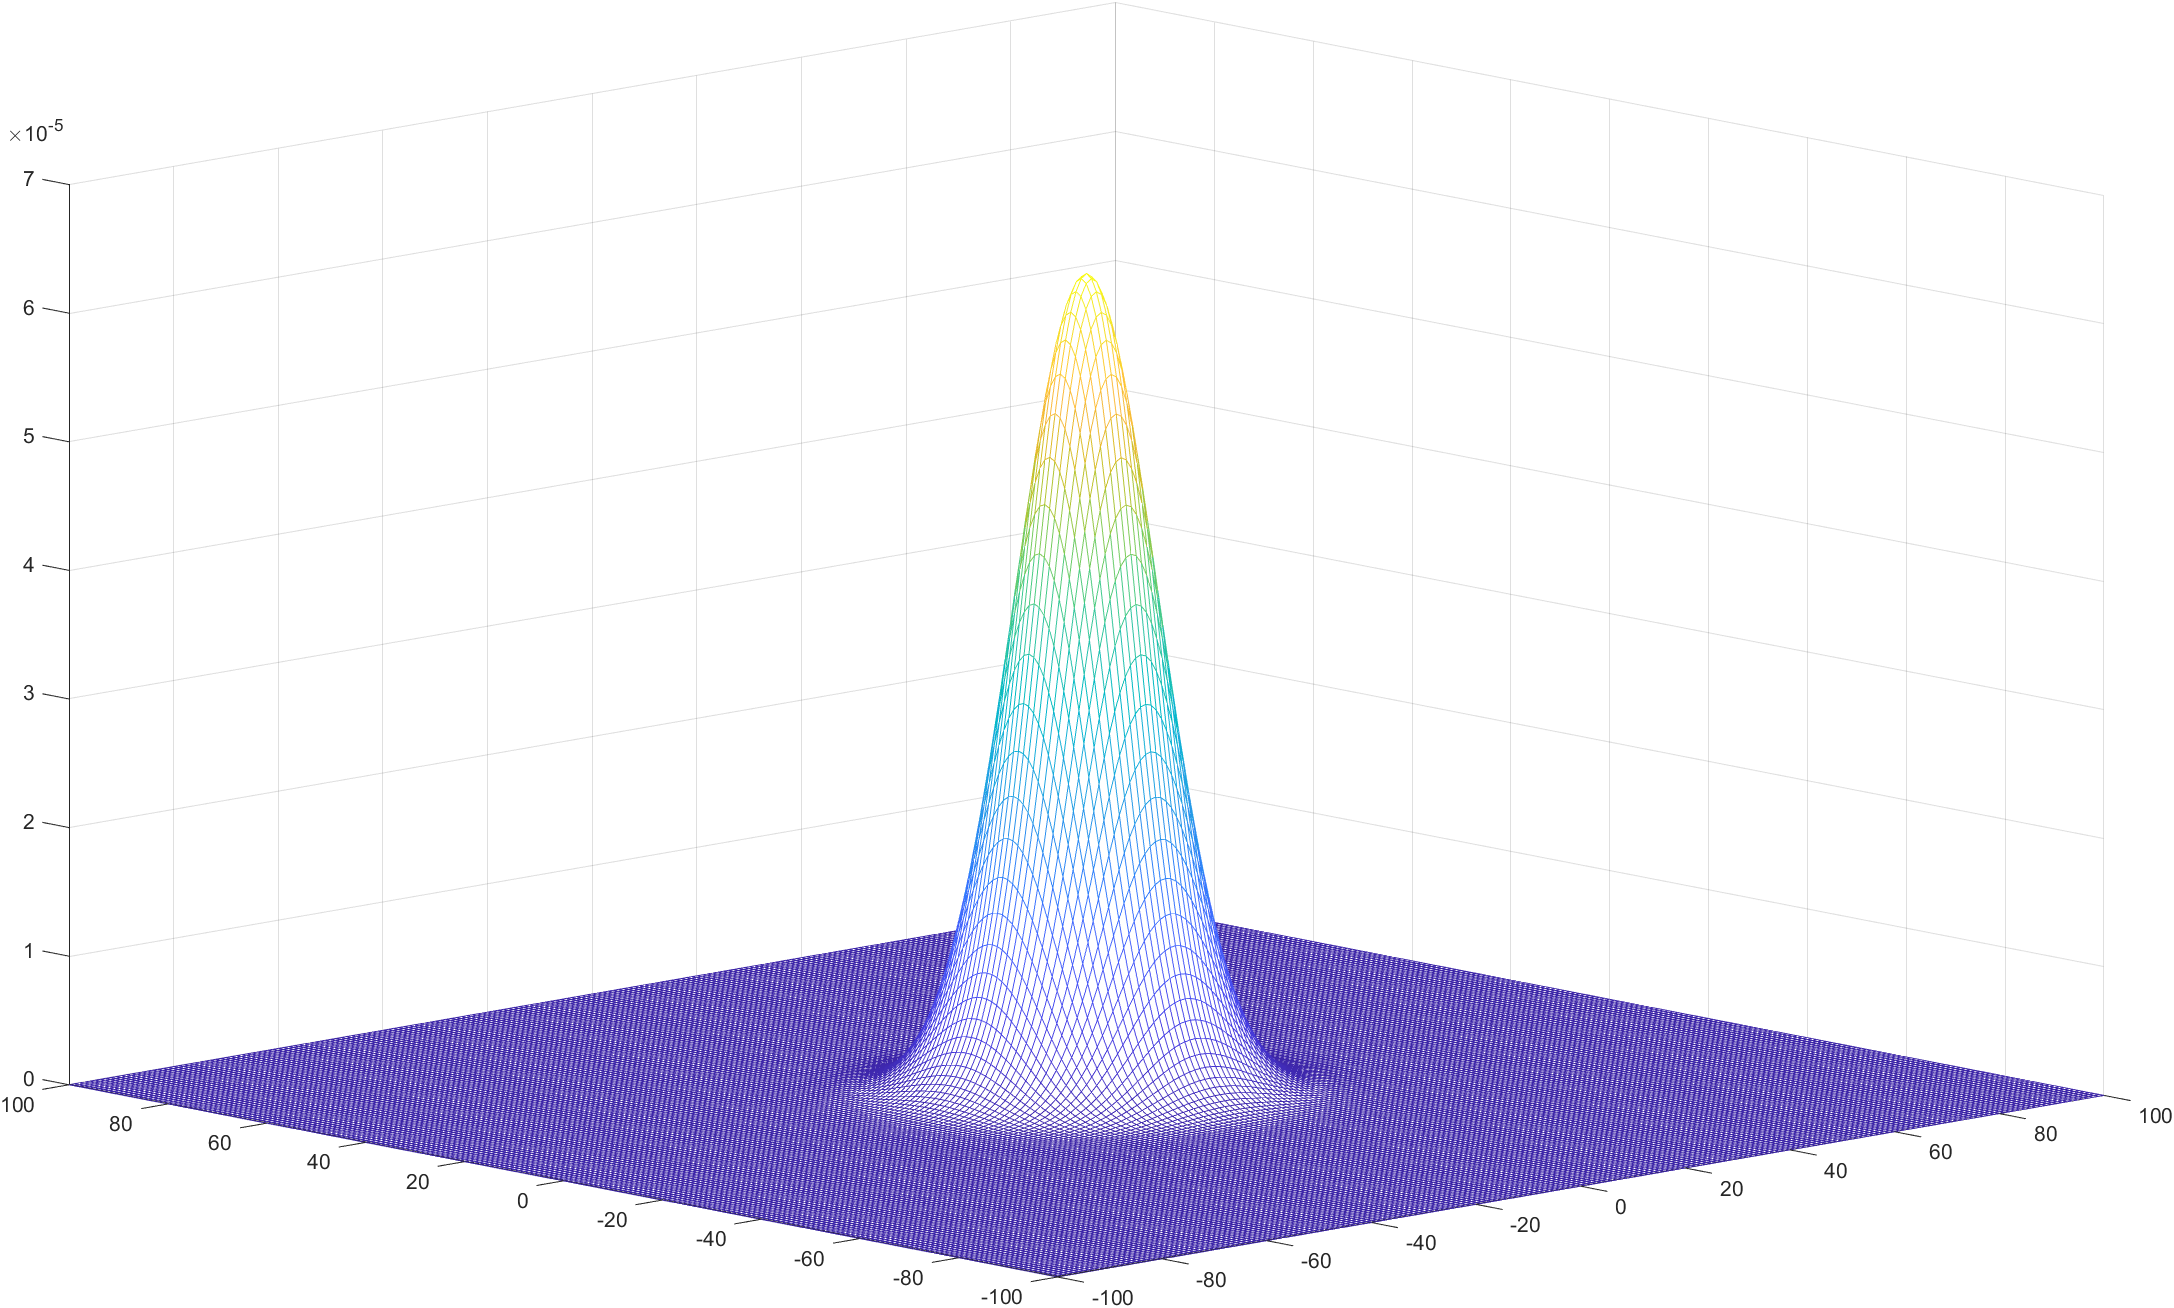
\includegraphics[width=7.5cm]{Fig/Gaussian.png}}
    \hspace{0.5in}
    \subfigure[并排图片示例2]{
        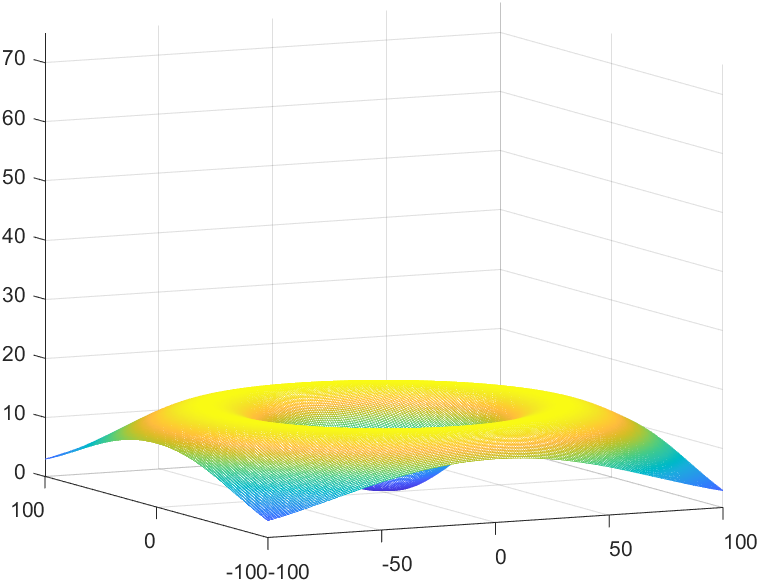
\includegraphics[width=7.5cm]{Fig/Maxwell.png}}
    \hspace{0.5in}
    \caption{并排图片}
\end{figure}

\section{思考题}

\begin{enumerate}
    \item 思考题1

    答: 啊对对对
    \item 思考题2

    答: 啊对对对
\end{enumerate}

\section{总结}

阿巴阿巴阿巴. 

\section{实验原始数据记录表}
见后附图. 

用以下指令轻松插入数据记录表. 
\begin{lstlisting}
\includepdf[pages={1-4}]{record.pdf}
\end{lstlisting}
\texttt{record.pdf}是导入的数据记录表的pdf文件, \texttt{pages=\{1-4\}}表示要包含的页码范围. 

\begin{figure}[htbp]
    \centering
    
\includegraphics[width=16cm]{Fig/511&509.png}
    \caption{最终解释权归511\&509科学院享有}
\end{figure}

\end{document}